%%%%%%%%%%%%%%%%%%%%%%%%%%%%%%%%%%%%%%%%%
% Beamer Presentation
% LaTeX Template
% Version 1.0 (10/11/12)
%
% This template has been downloaded from:
% http://www.LaTeXTemplates.com
%
% License:
% CC BY-NC-SA 3.0 (http://creativecommons.org/licenses/by-nc-sa/3.0/)
%
%%%%%%%%%%%%%%%%%%%%%%%%%%%%%%%%%%%%%%%%%



%----------------------------------------------------------------------------------------
%	PACKAGES AND THEMES
%----------------------------------------------------------------------------------------

%\documentclass[10pt]{beamer}
\documentclass[aspectratio=169]{beamer}

\mode<presentation> {

% The Beamer class comes with a number of default slide themes
% which change the colors and layouts of slides. Below this is a list
% of all the themes, uncomment each in turn to see what they look like.

%\usetheme{default}
%\usetheme{AnnArbor}
%\usetheme{Antibes}
%\usetheme{Bergen}
%\usetheme{Berkeley}
%\usetheme{Berlin}
%\usetheme{Boadilla}
%\usetheme{CambridgeUS}
%\usetheme{Copenhagen}
%\usetheme{Darmstadt}
%\usetheme{Dresden}
\usetheme{Frankfurt}
%\usetheme{Goettingen}
%\usetheme{Hannover}
%\usetheme{Ilmenau}
%\usetheme{JuanLesPins}
%\usetheme{Luebeck}
%\usetheme{Madrid}
%\usetheme{Malmoe}
%\usetheme{Marburg}
%\usetheme{Montpellier}
%\usetheme{PaloAlto}
%\usetheme{Pittsburgh}
%\usetheme{Rochester}
%\usetheme{Singapore}
%\usetheme{Szeged}
%\usetheme{Warsaw}

% As well as themes, the Beamer class has a number of color themes
% for any slide theme. Uncomment each of these in turn to see how it
% changes the colors of your current slide theme.

%\usecolortheme{albatross}
%\usecolortheme{beaver}
%\usecolortheme{beetle}
%\usecolortheme{crane}
%\usecolortheme{dolphin}
%\usecolortheme{dove}
%\usecolortheme{fly}
%\usecolortheme{lily}
%\usecolortheme{orchid}
%\usecolortheme{rose}
%\usecolortheme{seagull}
%\usecolortheme{seahorse}
%\usecolortheme{whale}
%\usecolortheme{wolverine}

%\setbeamertemplate{footline} % To remove the footer line in all slides uncomment this line
%\setbeamertemplate{footline}[page number] % To replace the footer line in all slides with a simple slide count uncomment this line

%\setbeamertemplate{navigation symbols}{} % To remove the navigation symbols from the bottom of all slides uncomment this line
}


%\setbeamertemplate{headline}
%{%
% \begin{beamercolorbox}{section in head/foot}
%\vskip1pt\insertnavigation{\textwidth}{}{}\vskip2pt
%  \end{beamercolorbox}
%}

\setbeamercolor{section in head/foot}{bg=lightgray} %set the top navigation bar background color
\setbeamertemplate{footline}[frame number] % set frame page number only
\usepackage{appendixnumberbeamer} % total will not include appendix frame numbers 

\beamertemplatenavigationsymbolsempty



\usepackage{graphicx} % Allows including images
% graphicx also allows for resizebox
% graphicx also allows for \scalebox
\usepackage{caption}
\usepackage{subcaption} % packgage for subcaption in subfigures
% The subfig and subcaption packages can not be used in cooperation with each other. Instead, you can usecaption package with subfig to add some flavor to the captions and subcaptions
\usepackage{bm} % make bold math symbols
\usefonttheme{professionalfonts}
%\usepackage{newtxtext,newtxmath} % for professional fond to load a Times Roman clone
\usepackage{tabularx} % extra features for tabular environment
\usepackage{booktabs} % Allows the use of \toprule, \midrule and \bottomrule in tables
\usepackage{adjustbox} % allows adjustbox
\usepackage{amsmath}  
\usepackage{amsfonts}
\usepackage{hyperref} % package for hyper link

% the following hypersetup makes link blue
\hypersetup{
  colorlinks   = true, %Colours links instead of ugly boxes
  urlcolor     = blue, %Colour for external hyperlinks
  linkcolor    = blue, %Colour of internal links
  citecolor   = blue %Colour of citations
}


\usepackage{float} % make the table H effective
\restylefloat{table}
\usepackage{color, colortbl}
\usepackage{booktabs} % package for tex professional table
\usepackage{mathtools} % package for \coloneqq
\usepackage{multirow} % multirow for intuition page.

% make pdf dark mode
%\usepackage{xcolor}
%\pagecolor[rgb]{0,0,0} %black
%\color[rgb]{0.5,0.5,0.5} %grey

\usepackage{pifont}% http://ctan.org/pkg/pifont
\newcommand{\cmark}{\ding{51}}%
\newcommand{\xmark}{\ding{55}}%



\usepackage{tikz} % graph in latex
\usetikzlibrary{positioning,arrows.meta} %tikz diagram
\usepackage{pgfplots}
\pgfplotsset{compat=newest} %this setting allow node to go to the correct place
\usepgfplotslibrary{fillbetween}

% use the tikz external library to cache tikz drawings
\usetikzlibrary{external}
\tikzexternalize[prefix=tikz/,optimize command away=\includepdf]


%\bibliography{bibliography}
%\usepackage[american]{babel}
%\usepackage{csquotes}
%\usepackage[style=apa]{biblatex}
%\DeclareLanguageMapping{american}{american-apa}
%\addbibresource{References.bib}

\usepackage{natbib} % package for citation


%\usepackage{subfigure} % subfigure package
%\captionsetup[subfigure]{labelformat=empty}
% The subfig and subcaption packages can not be used in cooperation with each other. Instead, you can usecaption package with subfig to add some flavor to the captions and subcaptions

%\usepackage{natbib} % package for citation

% define a comment line that does nothing to hide content
\newcommand{\comment}[1]{}
\newcommand{\lnb}[1]{%
  \ln\left(#1\right)%
}

\renewcommand{\baselinestretch}{1.0} %  scales the default interline space to 1.0 its default value. 

% define a comment that can scale the equation 
\newcommand\scalemath[2]{\scalebox{#1}{\mbox{\ensuremath{\displaystyle #2}}}}

%----------------------------------------------------------------------------------------
%	TITLE PAGE
%----------------------------------------------------------------------------------------

\title[The Traditional Finance Industry (``Tradfi'')]{\huge{The Traditional Finance Industry (``Tradfi'')} \\
\vspace{6mm}
\small{MGT 4074 Fintech \& Crypto Tokens, Spring 2025}
} % The short title appears at the bottom of every slide, the full title is only on the title page


%\subtitle{Presentation to Shanghai International Studies University}


\author[Joseph Hall]{Joseph Hall} % Your name
\institute[GT]{Georgia Institute of Technology} % Your institution as it will appear on the bottom of every slide, may be shorthand to save space
 % Your institution for the title page
 % Your email address
 
\date{August 27, 2025} 
 % Date, can be changed to a custom date if without date



%---------------------------------------------------------------------------
\begin{document}

\begin{frame}
\titlepage % Print the title page as the first slide
\end{frame}


%----------------------------------------------------------------------------------------

%	PRESENTATION SLIDES
%----------------------------------------------------------------------------------------

%-----------------------------------------------



%---------------------------------------------------------------------
%---------------------------------------------------------------------
%\section*{Introduction}
% When I comment the introduction section, fewer sections show up in navigation
%---------------------------------------------------------------------
%---------------------------------------------------------------------

\begin{frame}{Welcome}

\begin{center}

    No quiz today! Roll Call instead. \\ 
    \vfill 
    For next class (after Labor Day), please read: \\
        ``Bank Runs, Deposit Insurance, and Liquidity'' \\
    By Diamond and Dybvig \\
    \hyperlink{https://www.journals.uchicago.edu/doi/abs/10.1086/261155}{https://www.journals.uchicago.edu/doi/abs/10.1086/261155}
    \vfill 
    This is our longest and hardest reading yet, but you have 7 full days to do it, and I will instruct you on how to read this paper. 
\end{center}
    
\end{frame}


\begin{frame}{Schedule Today}

\begin{itemize}
    \item In the News: Lisa Cook and Federal Reserve Independence 
    \item Guided Discussion: Seeing Like a Bank 
    \item How to Read an Economic Theory Paper 
    \item The Traditional Financial System 
    \begin{itemize}
        \item Debt and Equity Contracts 
        \item Market Structure
        \item Financial Intermediaries 
        \item Transaction Costs 
        \item Asymmetric Information 
        \item Moral Hazard 
        \item Deposit Insurance 
    \end{itemize} 
\end{itemize}
    
\end{frame}

\begin{frame}{In the News: Fed Independence}

\begin{center}
    
\includegraphics[height = .9\textheight]{trump.png}
\end{center}
    
\end{frame}

\begin{frame}{In the News: Fed Independence}

\textbf{Q}: What do we mean when we say ``\textbf{Fed Independence}''? Why is it important for monetary policy? \pause \vfill 
\textbf{A.1}: The Federal Reserve is called ``Independent'' because the governors have long, overlapping terms, and cannot be fired without \textbf{``cause''}. \\ \pause 
\textbf{A.2}: Independence is important so that short-term politicians do not abuse \emph{seignorage} and debase the currency by creating too much money \\ \pause 
\textbf{Q:} What does it mean to fire Lisa Cook ``with cause''? \\ 
\textbf{A:} ``With cause'' tends to mean due to gross misconduct or fraud. Governor Cook has announced she will appeal the firing in court. Federal courts will now decide whether the alleged misrepresentation she made on her mortgage application qualified as cause for firing. The markets will watch closely. 
    
\end{frame}

\begin{frame}{Market Reactions}

\begin{center}
    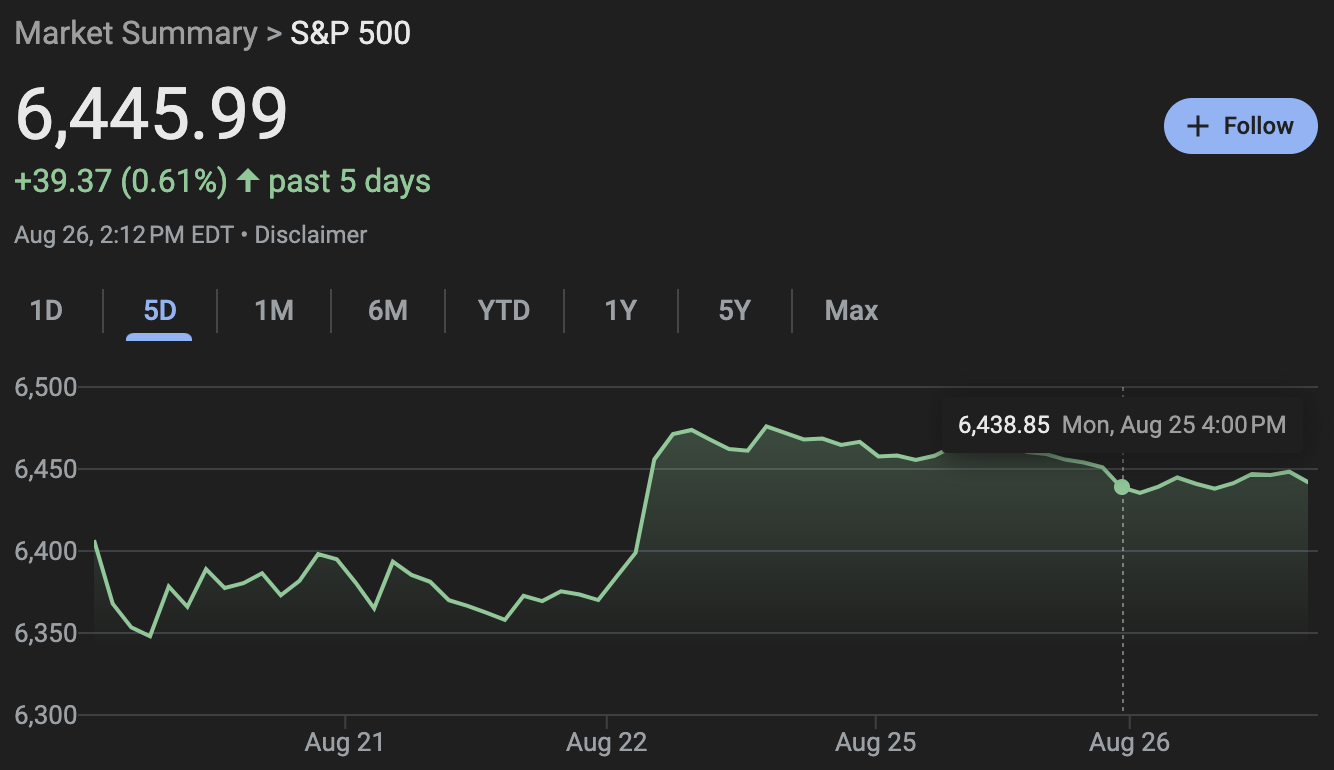
\includegraphics[width = .8\textwidth]{sp500.png}
\end{center}
\begin{itemize}
    \item Equities priced in dollars have not moved (is this expected?) 
\end{itemize}
    
\end{frame}


\begin{frame}{Market Reactions}

\begin{center}
    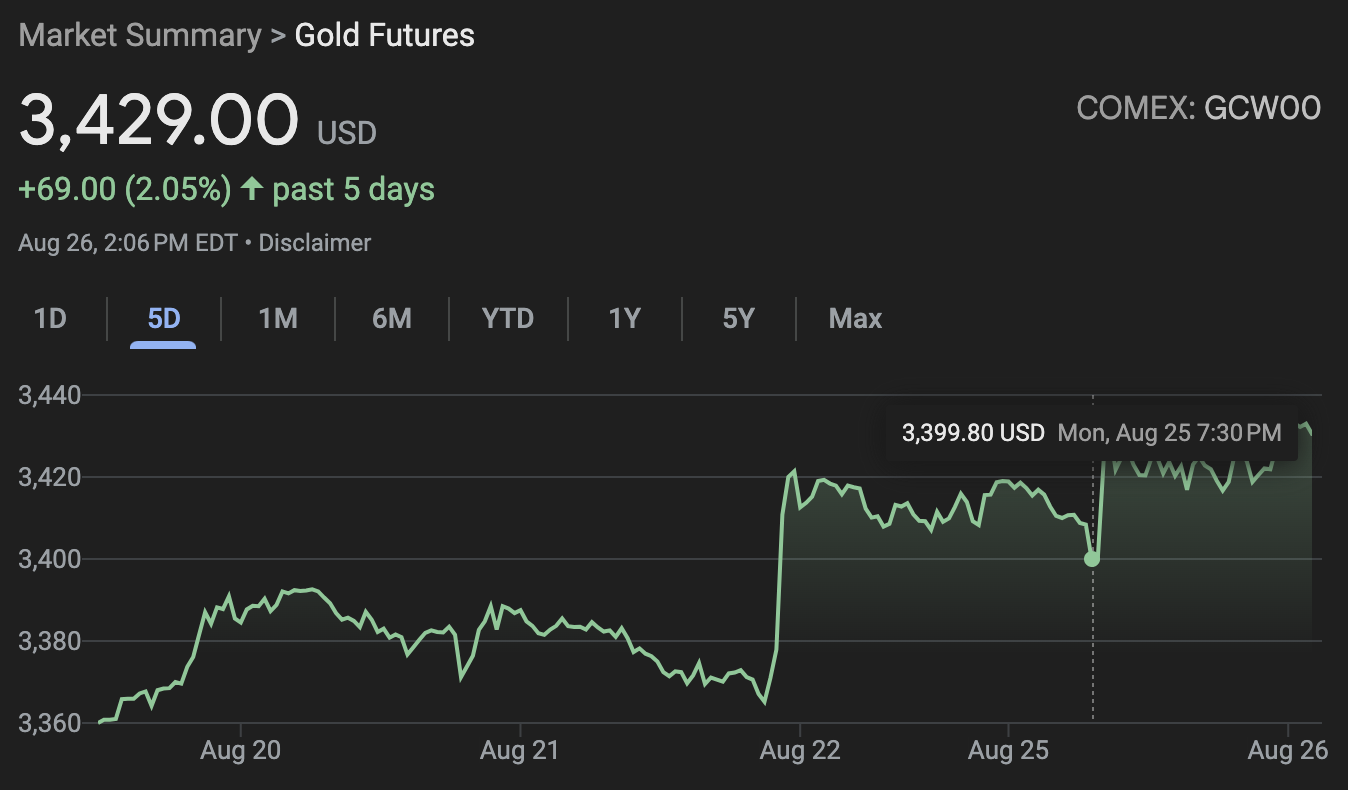
\includegraphics[width = .8\textwidth]{gold.png}
\end{center}
\begin{itemize}
    \item Gold is up slightly (is this expected?) 
\end{itemize}
    
\end{frame}



\begin{frame}{Seeing Like a Bank}

\begin{itemize}
    
    \item What is ``tiered customer support''? What trade-offs does a bank face when implementing tiered support? \pause 

    \item The essay likens bank systems to ``sedimentary layers.'' What does that mean? \pause 

    \item Why do regulations require secrecy in Suspicious Activity Reports? \pause 

    \item If some customers never grasp basic banking math, is the failure theirs, society’s, or the bank’s? How should banks respond? 
    
\end{itemize}
    
\end{frame}


\begin{frame}{Seeing Like a Bank: My Answers}

This is how I, personally, would answer each of these discussion questions: 

\begin{itemize}
    
    \item ``Tiers'' of customer support act as a funnel where customers are \textbf{assumed to be unsophisticated and financially illiterate until proven otherwise}. This can improve efficiency, but harm service quality especially for a bank's highest-value customers. 
    \pause 

    \item Banking technology systems are like ``sedimentary layers'' in that new systems are often grafted onto, rather than replace, old systems. \pause 

    \item Suspicious Activity Reports must be generated when a customer may be a criminal. Therefore banks are sometimes prohibited by law from serving their customers transparently. \pause 

    \item Low financial literacy persists across society and gives sophisticated counterparties ample opportunities to take advantage. My opinion? Banks should deal in good faith and build reputations for honesty and quality, not count on optimized contract language to immunize them from lawsuits. 
    
\end{itemize}
    
\end{frame}




\begin{frame}{How to read an economic theory paper}

My system: 
\begin{enumerate}
    \item Print out the paper. block out one hour to read it with \textbf{no other screens or notifications}, just a notepad and pen 
    \item Copy down key terms in the abstract that you don't understand 
    \item Read through the paper, copying down any \textbf{definitions of the key terms} as you encounter them
    \begin{itemize}
        \item Take as many one-hour sessions as you need with breaks in between. The sessions should be uninterrupted. 
    \end{itemize}
    \item At the end, re-read the abstract, the intro, and the conclusion 
    \item Write down the \textbf{main result} of the paper (the key argument which is proven true in the body of the paper) in two sentences or fewer, in your own words. Bookmark the page in the paper where you believe the statement of the key result is given. 
\end{enumerate}

    
\end{frame}



%------------------------------------------------
%------------------------------------------------
\begin{frame}
\frametitle{Debt and Equity Contracts}

\begin{itemize}
    \item \textbf{Debt}: a contract to repay a \textbf{fixed dollar amount} on a specific schedule 
    \begin{itemize}
        \item Failing to pay a debt contract results in \textbf{corporate bankruptcy}: a court gives the senior debt-holders complete control and ownership of the company (their debt is \emph{converted} into equity)  \pause 
        \item US Treasuries are considered the world's safest debt, and the US Treasury market is the world's largest debt market (why?) \pause 
    \end{itemize}
%\vspace{-3mm}
%-----------------------------------------------
%\begin{figure}[H]
%    \resizebox{4in}{1in}{%
    %\resizebox{\textwidth}{!}{%
%    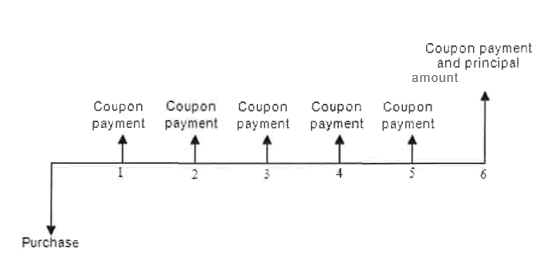
\includegraphics[]{Figure/LongTermDebt_Cashflow.png}
%    } %end of resizebox
%-----------------------------------------------
% Figure setting: caption and label
%-----------------------------------------------
%\caption{}
%\label{fig:ModelIntuition_Graphs}
%\end{figure}
%-----------------------------------------------
%\vspace{-1mm}

    \item \textbf{Equity}: a contract to pay a \textbf{percentage} of profits after debt is repaid 
    %\item \textbf{Compared to debt}:
    \begin{itemize}
        \item Equity contracts traditionally include \textbf{control rights} over the company (e.g. voting on Board members), to ensure the company's officers do not expropriate profits 
        %\item Disadvantage: an equity holder is a residual claimant; that is, the corporation must pay debt holders before paying equity holders.
        %\item Advantage: benefit directly from any increases in the corporation’s profitability or asset value. In contrast, debt payments are fixed
    \end{itemize}
\end{itemize}\pause \smallskip 

The theory of \textbf{Townsend} (1979) argues that debt and equity are \emph{THE optimal combination of contracts} between investors and entrepreneurs who face information asymmetry, when it is costly for investors to verify the reports from entrepreneurs. 

\end{frame}
%------------------------------------------------

\begin{frame}{Discussion on Debt and Equity}

    \begin{itemize}
        \item \textbf{Q}: Can you think of any popular financial contracts that are not debt or equity? \pause 
        \begin{itemize}
            \item Prediction (gambling) markets trade ``\textbf{arrow securities}'': \$1 if prediction true, \$0 if false (same with insurance markets)
            \item \textbf{Variable annuities}: retirement funds that combine debt- and equity-like features 
            \item Credit cards include ``\textbf{revolving debt}'' contracts governed by \textbf{credit limits} and interest charged on unpaid (``revolving'') balances 
        \end{itemize}
        \vfill 
        \item \textbf{Q}: Do you have any entrepreneurial ideas? Would you seek outside financing? If so, in what form? \pause 
        \vfill 
        \item \textbf{Q}: If you wanted to raise debt or equity from the public, do you know what you'd need to do? \pause 
        \begin{itemize}
            \item Legally incorporate a company with an independent board of directors 
            \item File a ``Prospectus'' with the SEC including audited financial statements 
            \item Find a venue to sell your shares to, either via an investment bank (an ``IPO'') or a securities exchange directly (a ``direct listing'') 
            \item \textbf{Skipping these steps is illegal under federal law!}
        \end{itemize}
    \end{itemize}
    
\end{frame}




%------------------------------------------------
\begin{frame}
\frametitle{Structure of Financial Markets}

Most financial markets can be classified as either \textbf{Money Markets} or \textbf{Capital Markets}: 
\smallskip 
\textbf{Money market}:
\begin{itemize} 
    \item \textbf{Definition}: a financial market in which only short-term debt instruments (original maturity less than one year) are traded. 
    \item \textbf{Usage}: corporations, banks, and households store excess money in these instruments to earn a bit of interest while staying perfectly \textbf{liquid} 
\end{itemize}
\smallskip 
\textbf{Capital market}
\begin{itemize} 
    \item \textbf{Definition}: a financial market in which longer-term debt instruments (original maturity one year or greater) and equity instruments are traded
    \item \textbf{Usage}: investors with long time horizons (such as pension funds or young high earners) invest in capital markets to maximize long-run return 
\end{itemize}


\end{frame}
%------------------------------------------------


%------------------------------------------------
\begin{frame}
\frametitle{Structure of Financial Markets}

\textbf{Primary Markets}: \textbf{new issues of a security (a bond or a stock)}  are sold.
\begin{itemize}
    \item Often take place privately between the issuer and a financial institution such as an investment bank 
    \item Investment banks \textbf{underwrite} securities: they buy a corporation’s securities at a negotiated price, then offer them to the public (this is called an \textbf{Initial Public Offering (IPO)} 
\end{itemize} \pause 

\medskip 

\textbf{Secondary Markets}: previously issued securities (stocks and/or bonds) are traded
\begin{itemize}
    \item \textbf{Example}: The New York Stock Exchange and NASDAQ (National Association of Securities Dealers Automated Quotation System)
    %\item \textbf{Benefits}: (1) liquidity (easier to sell financial instruments to raise cash), and (2) price discovery 
    \item Key market participants: 
    \begin{itemize}
        \item \textbf{Brokers}: match buyers with sellers of securities, earning percentage \textbf{commission}.
        \item \textbf{Dealers}: intermediate between buyers and sellers by trading securities, earning \textbf{profit from price differences}.
        \item Many financial institutions perform both functions and are ``\textbf{broker-dealers}''
    \end{itemize}
\end{itemize}


\end{frame}
%------------------------------------------------

%------------------------------------------------
\begin{frame}
\frametitle{Structure of Financial Markets}

\textbf{Secondary markets}: (1) Exchange and (2) over-the-counter (OTC) market \\
\smallskip 
\textbf{Exchange}:
\begin{itemize} 
    \item \textbf{Definition}: buyers and sellers of securities (or their agents or brokers) meet in one central location to conduct trades. 
    \item \textbf{Features}: via physical location and computers, highly competitive, more regulated
    \item \textbf{Examples}: New York Stock Exchange for stocks and the Chicago Board of Trade for Commodities
\end{itemize}
\smallskip 
\textbf{Over-the-counter (OTC) market}
\begin{itemize}
    \item \textbf{Definition}: \textbf{Dealers} at different locations who have an inventory of securities stand ready to buy and sell securities “over the counter” to \textbf{anyone} who comes to them and is willing to accept their prices
    \item \textbf{Features}: via computers, very competitive, larger amount, less regulated
    \item \textbf{Examples}: markets for U.S. government bonds, negotiable certificates of deposit, federal funds, and foreign exchange. 
\end{itemize}


\end{frame}
%------------------------------------------------




%------------------------------------------------
\begin{frame}
\frametitle{Structure of Financial Markets}

%\textbf{Money Market Instruments}: 
\vspace{-2mm}
%-----------------------------------------------
\begin{figure}[H]
    \resizebox{5.6in}{2.6in}{%
    %\resizebox{\textwidth}{!}{%
    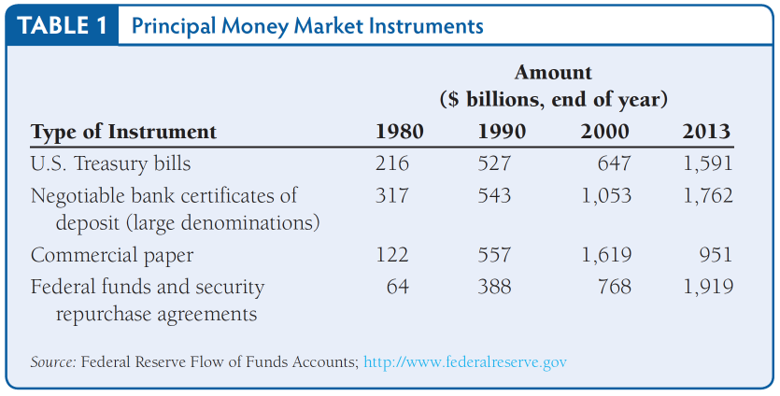
\includegraphics[]{Figure/MoneyMarketInstruments.png}
    } %end of resizebox
%-----------------------------------------------
% Figure setting: caption and label
%-----------------------------------------------
%\caption{}
%\label{fig:ModelIntuition_Graphs}
\end{figure}
%-----------------------------------------------


\end{frame}
%------------------------------------------------




%------------------------------------------------
\begin{frame}
\frametitle{Structure of Financial Markets}

%\textbf{Capital Market Instruments}: 
\vspace{-2mm}
%-----------------------------------------------
\begin{figure}[H]
    \resizebox{5.6in}{2.6in}{%
    %\resizebox{\textwidth}{!}{%
    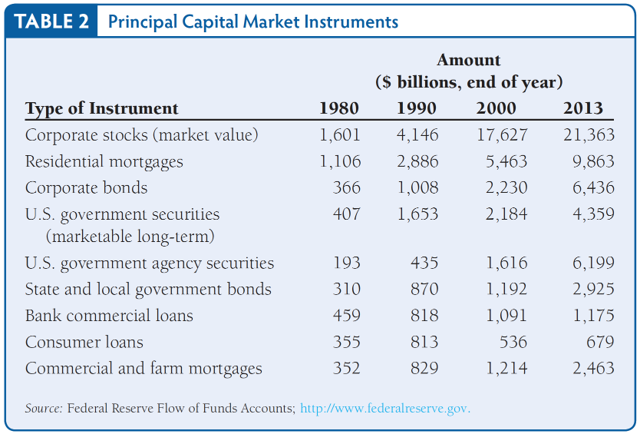
\includegraphics[]{Figure/CapitalMarketInstruments.png}
    } %end of resizebox
%-----------------------------------------------
% Figure setting: caption and label
%-----------------------------------------------
%\caption{}
%\label{fig:ModelIntuition_Graphs}
\end{figure}
%-----------------------------------------------


\end{frame}
%------------------------------------------------



\subsection{Financial Intermediaries}


%------------------------------------------------
\begin{frame}
\frametitle{Financial Intermediaries}

%\textbf{Capital Market Instruments}: 
\vspace{-6mm}
%-----------------------------------------------
\begin{figure}[H]
    \resizebox{5.6in}{2.9in}{%
    %\resizebox{\textwidth}{!}{%
    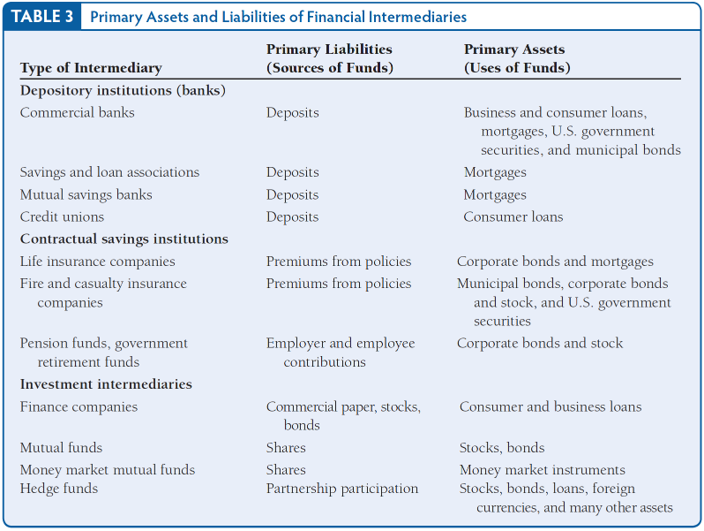
\includegraphics[]{Figure/FinancialIntermediaries.png}
    } %end of resizebox
%-----------------------------------------------
% Figure setting: caption and label
%-----------------------------------------------
%\caption{}
%\label{fig:ModelIntuition_Graphs}
\end{figure}
%-----------------------------------------------


\end{frame}
%------------------------------------------------




%------------------------------------------------
\begin{frame}
\frametitle{Financial Intermediaries}

%\textbf{Capital Market Instruments}: 
\vspace{-6mm}
%-----------------------------------------------
\begin{figure}[H]
    \resizebox{5.6in}{2.9in}{%
    %\resizebox{\textwidth}{!}{%
    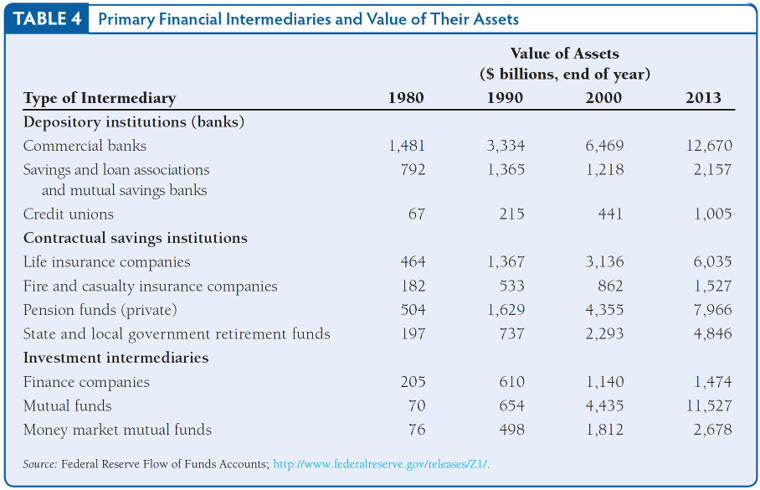
\includegraphics[]{Figure/FinancialIntermediaries_MarketSize.png}
    } %end of resizebox
%-----------------------------------------------
% Figure setting: caption and label
%-----------------------------------------------
%\caption{}
%\label{fig:ModelIntuition_Graphs}
\end{figure}
%-----------------------------------------------


\end{frame}
%------------------------------------------------



\begin{frame}{Business Models of Financial Intermediaries}
\begin{center}
    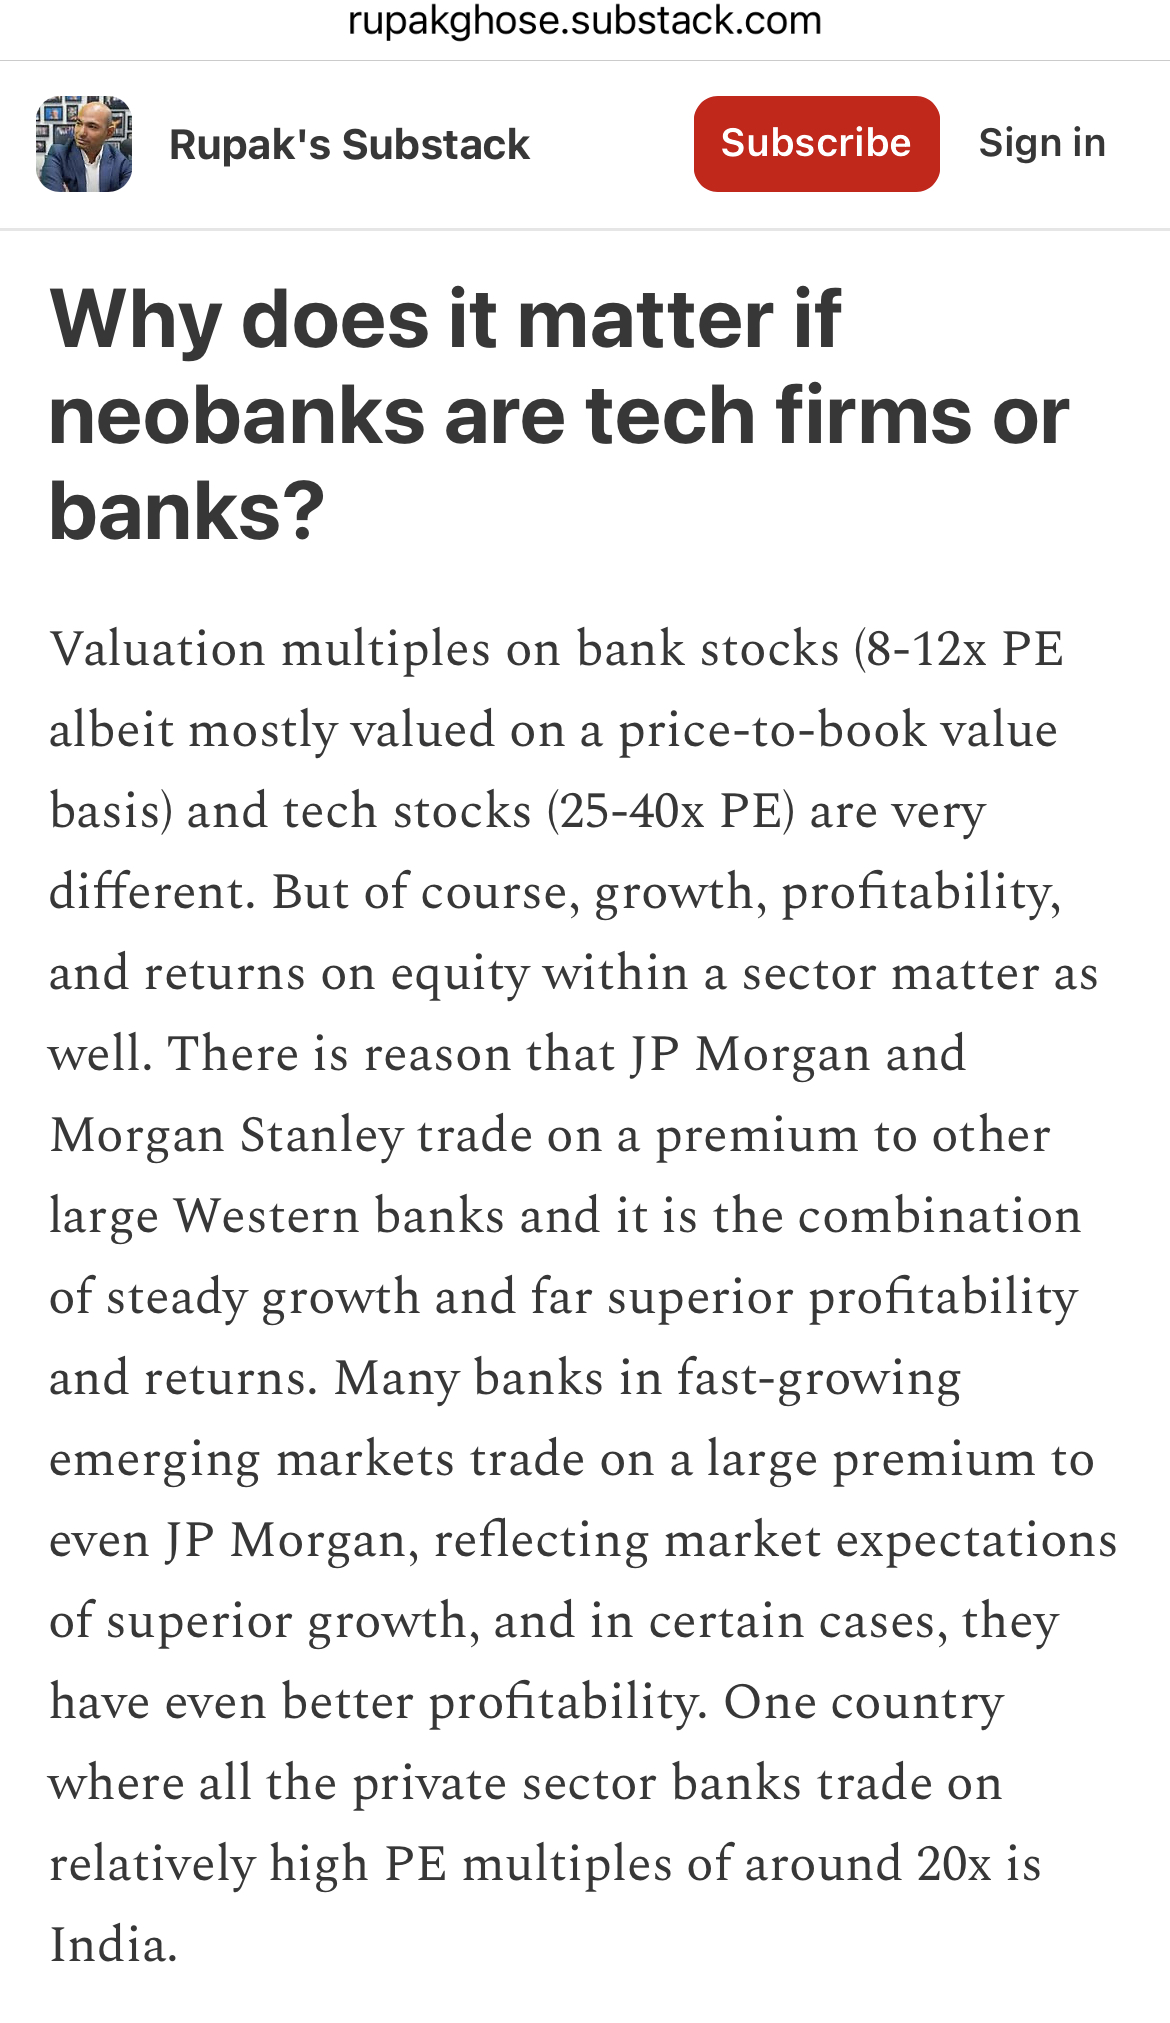
\includegraphics[scale = 0.1]{Figure/original-F9E1A12F-36C4-4EB2-91A0-740A9E829D83.jpeg}

\end{center}

\end{frame}



\begin{frame}{Welcome to Class}

\begin{center}
    Today is Wednesday, September 3 \\ 
    Midterm Exam \#1 is \textbf{Monday, September 8} \\ 
    The Practice Exam is on Canvas. 
\end{center}
    
\end{frame}


\begin{frame}{Schedule for Today}

\begin{itemize}
    \item Quiz Review: Liquidity, Deposit Insurance and Bank Runs 
    \item In the News: Tornado Cash, Luna-Terra Founders Guilty in Court 
    \item The Traditional Financial System: 
    \begin{itemize}
        \item Transaction Costs 
        \item Asymmetric Information 
        \begin{itemize}
            \item Adverse Selection 
            \item Moral Hazard 
            \item A Story from my Grandfather 
            \item The Paradox of Information, aka the ``No-Trade Theorem'' 
        \end{itemize}
        \item Tools for Solving Asymmetric Information
        \item Deposit Insurance 
        \item Banking Crises and the Real Economy 
    \end{itemize}

\end{itemize}
    
\end{frame}

\begin{frame}{Quiz Review}

1.	What is the source of risk in the model? \pause \\ 

Answer: Some agents will need to withdraw their money early, at a time when their money is invested in a long-term illiquid project  
    
\end{frame}

\begin{frame}{Quiz Review}

2.	What incentive does the bank have to invest in illiquid assets, so that not everybody can withdraw their money every period?   \pause \\ 

Answer: There is a productive technology that gives a higher rate of return, but only if the capital is locked up for two periods 
    
\end{frame}

\begin{frame}{Quiz Review}

3.	True or False: A market with only the uninsured deposit contract has a unique equilibrium which is a bank run    \pause  \\ 

Answer: False. Without deposit insurance, multiple equilibria exist: you will run on the bank if others do, and vice versa. 
    
\end{frame}

\begin{frame}{Quiz Review}

4.	What is the role of deposit insurance in the model?     \pause \\ 

Answer: It eliminates the incentive for agents to ever withdraw early when they don’t need to. No incentive for a bank run? No run materializes. The insurance is an effective deterrent even though it never pays out in equilibrium! 
    
\end{frame}



\begin{frame}{In the News: Feds Bust Tornado Cash, Luna-Terra}

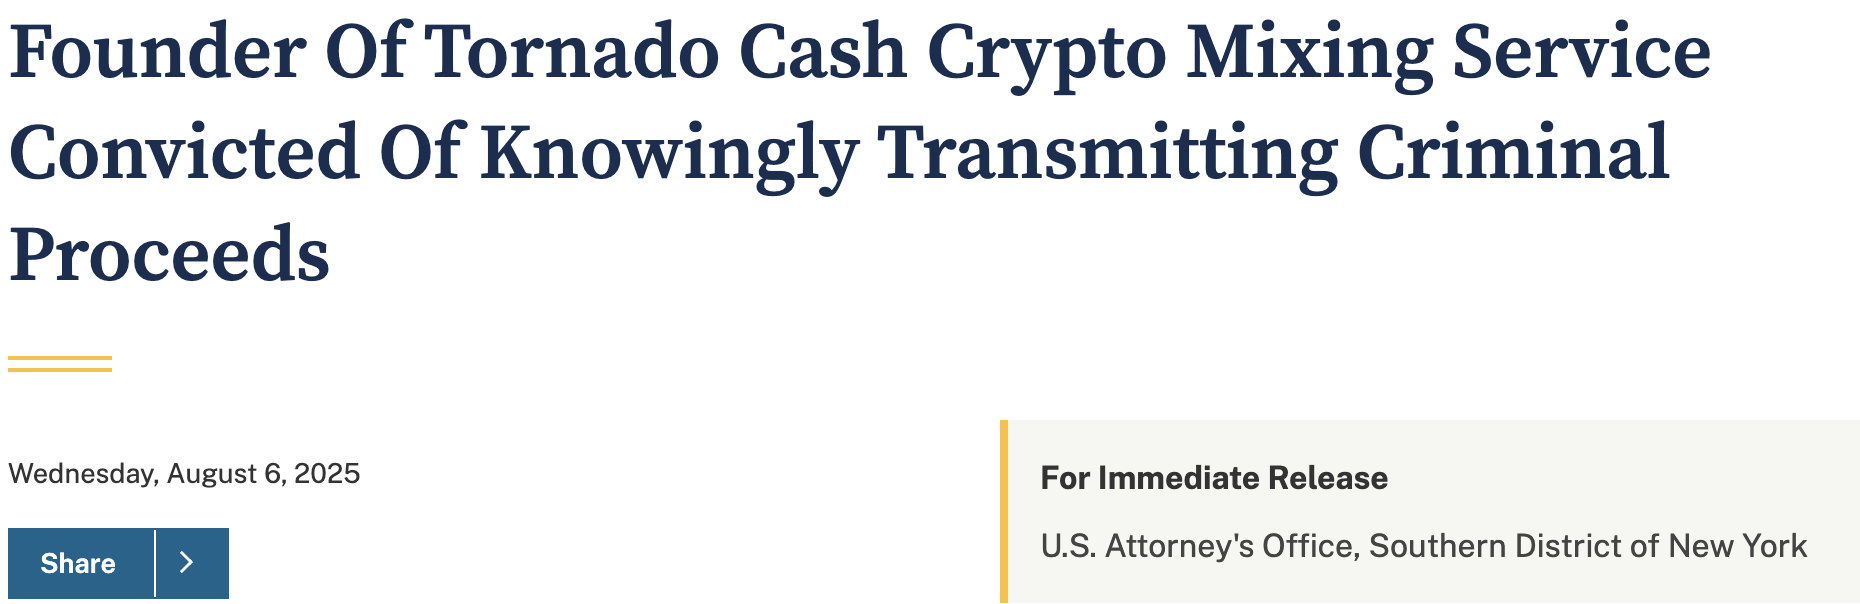
\includegraphics[height = .45\textheight]{tornado.png} \\ 

\includegraphics[height = .45\textheight]{dokwon.png}

\end{frame}

\begin{frame}{Do Not Do This:}

\begin{quote}
    Tornado Cash advertised to customers that it provided untraceable and anonymous financial transactions, and STORM continued to provide this service with knowledge that Tornado Cash was transmitting large volumes of criminal proceeds.  As proven at trial, STORM was personally aware of numerous instances in which criminals transmitted proceeds of criminal exploits using Tornado Cash, totaling more than $\$1$ billion in criminal proceeds.
\end{quote}
\pause Maximum potential prison sentence: 5 years 
    
\end{frame}


\begin{frame}{Do Not Do This Either:}

\begin{quote}
    KWON touted Terraform as a self-contained and decentralized financial world that leveraged proprietary blockchain technology to offer its own cryptocurrencies, payment system, stock market, and savings bank.  In reality and unbeknownst to Terraform investors and users, the core suite of Terraform products did not work as advertised and had been manipulated to create the illusion of a functioning and decentralized financial system.
\end{quote}
\pause Maximum potential prison sentence: 25 years 

    
\end{frame}

%------------------------------------------------
\subsection{Transaction Costs}
%------------------------------------------------
%------------------------------------------------

\begin{frame}
\frametitle{Transaction Costs}


\textbf{Transaction costs hinder flow of funds to people with productive investment opportunities}. Example: suppose you have \$5000 to invest 
\begin{itemize}
        %\item Stock market: can only buy a small number of shares
        \item Can you directly identify an entrepreneur in need of \$5,000 and enter a contract with them? \pause 
        \item Debt market: many contracts have \emph{minimum} denominations at \$10,000 or above 
        \item If you find a debt contract at \$5,000 you can buy directly, you will be under-diversified: ``all eggs in one (or few) baskets".
\end{itemize}  \pause 


\medskip 

\textbf{Financial intermediaries reduce transaction costs}
\begin{itemize}
    \item Economies of scale: average cost per dollar decreases with scale
    \begin{itemize}
        \item Example: Mutual Funds 
    \end{itemize}
    \item Develop expertise to lower transaction costs
    \begin{itemize}
        \item Robinhood and similar brokers charge zero transaction fees. 
    \end{itemize} 
\end{itemize}




\end{frame}

%------------------------------------------------


\subsection{Asymmetric Information: Adverse Selection and Moral Hazard}

%------------------------------------------------

\begin{frame}
\frametitle{Asymmetric Information}
\vspace{-2mm}
\textbf{Asymmetric Information}: 
\begin{itemize}
    \item Definition: when one party’s \textbf{insufficient knowledge} about the other party makes it hard to make accurate decisions
    \item Example: managers of a corporation know better information about how well their business is doing than stockholders do. \pause 
\end{itemize}

\textbf{Consequence of Asymmetric Information}: can lead to entire markets \emph{unraveling}! 
\begin{itemize}
    \item \textbf{Adverse selection}
    \begin{itemize}
        \item Definition: problem that occurs \textbf{before} a transaction occurs.
        \item Example: Big risk takers are the most eager to take out loans. Consequently, lenders might decide not to make any loans, even though good credit risks can be found. \pause 
    \end{itemize}
    \item \textbf{Moral Hazard}
    \begin{itemize}
        \item Definition: problem that occurs \textbf{after} a transaction occurs.
        \item Example: \textbf{After} a loan is initiated, the borrower might engage in activities that are undesirable/immoral (high risk, or in personal interest). Consequently, lenders might decide not to make any loans in the first place.
    \end{itemize}
\end{itemize}
%-----------------------------------------------

\vspace{-6mm}



\end{frame}

%------------------------------------------------


\begin{frame}{Examples of adverse selection and moral hazard}

Who can think of examples of \textbf{adverse selection?} \pause 

\begin{itemize}
    \item \textbf{Financing education with equity}: students who know they will be high earners are the least willing to surrender a percentage of their future earnings 
    \item \textbf{Medical insurance}: healthy people will not buy it if they know it's a bad deal for them 
\end{itemize}

\pause 

Who can think of examples of \textbf{moral hazard}? \pause 

\begin{itemize}
    \item \textbf{Medical insurance}: if medical care is free at the point of delivery, people (or their doctors) might order more procedures of questionable benefit 
    \item \textbf{Corporate debt/limited liability}: A company with \$100,000 in assets but \$100,000 in debt might take excessive risks, knowing that they get the upside but debtholders would face the downside 
\end{itemize}
    
\end{frame}




%------------------------------------------------

\begin{frame}
\frametitle{\large{George Akerlof (1970): 2001 Nobel Prize}}



\vspace{-2mm}
%-----------------------------------------------
\begin{figure}[H]
    \resizebox{1in}{1.6in}{%
    %\resizebox{\textwidth}{!}{%
    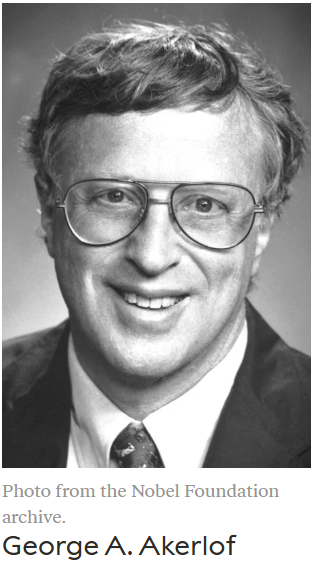
\includegraphics[]{Figure/Akerlof_2001NobelPrize.png}
    } %end of resizebox
%-----------------------------------------------
% Figure setting: caption and label
%-----------------------------------------------
%\caption{}
%\label{fig:ModelIntuition_Graphs}
\end{figure}
%-----------------------------------------------

%\textbf{2001 Nobel Prize in Economic Science: Award for George Akerlof}

\vspace{-4mm}
%-----------------------------------------------
\begin{figure}[H]
    \resizebox{5in}{1.1in}{%
    %\resizebox{\textwidth}{!}{%
    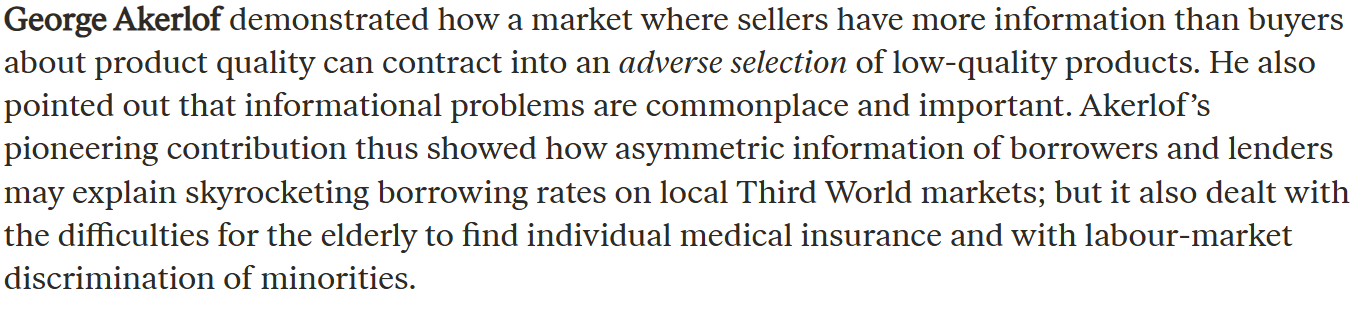
\includegraphics[]{Figure/Akerlof_2001NobelPrize_Award Speech.png}
    } %end of resizebox
%-----------------------------------------------
% Figure setting: caption and label
%-----------------------------------------------
%\caption{}
%\label{fig:ModelIntuition_Graphs}
\end{figure}
%-----------------------------------------------



\end{frame}

%------------------------------------------------

%------------------------------------------------

\begin{frame}
\frametitle{Adverse Selection in used-car market}


\textbf{\textcolor{red}{``Adverse selection"}} was first formulated by \textbf{George Akerlof (2001 Economic Nobel Prize)} in used-car market
\begin{itemize}
    \item \textbf{Two types of used cars}: 
    \begin{itemize}
        \item good (``peach"), fair value \$2000, probability: 50\%
        \item bad (``lemon"), fair value \$1000, probability: 50\%
    \end{itemize}
    \item \textbf{Asymmetric information}: the seller knows all, the buyer only knows probability  \pause 
    \item \textbf{Consequence: market will be \textcolor{red}{``adversely selected"}}
    \begin{itemize}
        \item The buyer only wants to pay: \$1000 * 0.5 + \$2000 * 0.5 = \$1500.  \pause 
        \item Given buyer's willingness to pay (\$1500), \textbf{``peach" owners do not want to sell and exit the market. Only ``lemon" owners stay}.  \pause 
        \item Expecting the above situation, only ``peach" are sold at \$1000. 
    \end{itemize}
\end{itemize}

\medskip 

Summary: since sellers of good cars (``peach") have been driven out of the market \textbf{in favor of bad cars (``lemon")}, the market has become \textbf{\textcolor{red}{“adversely selected”}}


\end{frame}

%------------------------------------------------



\begin{frame}{A story from my grandfather}

\begin{quote}
    ``If you walk into a bar, and a man offers you a \$10 bet that a fish will jump out of that barrel and spit in your eye..''
\end{quote} 

\textcolor{red}{What do you do?}  \pause 

\begin{quote}
    ``You do not take that bet. For if you do, as sure as you stand there, that fish will jump out of that barrel and spit in your eye, and you will lose \$10.''
\end{quote} 

-My grandfather TR Peterson 
    
\end{frame}



\begin{frame}{The Paradox of Information, aka ``No-Trade Theorem''}

\hyperlink{https://www.jstor.org/stable/1805228}{Grossman \& Stiglitz (1980)} make only two important assumptions: 

\begin{itemize}
    \item Some people know more than others what an asset's price should be 
    \item Everyone's preferences are the same: they only care about money \pause 
\end{itemize} \vfill 

With that, they prove that \emph{no trade should ever take place}! \pause \\
Intuition: the fact that your counterparty wants to trade with you is sufficient to know that you \emph{don't}!\\ \emph 
What do we learn from this? Trade must be justified by different \emph{preferences}, not by different \emph{information}


\end{frame}



%------------------------------------------------

\begin{frame}
\frametitle{Tools for Solving Asymmetric Information}



\textbf{Tools 1. Private production and sale of information}
\begin{itemize}
    \item \textbf{Hire firms for information production}: 
    \begin{itemize}
        \item \textbf{Example}: Standard and Poor’s, Moody’s, and Value Line gather information on firms’ balance sheet positions and investment activities and sell them to subscribers \pause 
    \end{itemize}
    \item \textbf{\textcolor{red}{Free-rider problem}}
    \begin{itemize}
        \item \textbf{Definition}: when people who do not pay for information take advantage of the information that other people have paid for
        \item \textbf{Example}: mutual fund A pays for S\&P and buys good stocks. Price of good stocks rises until all stocks are fairly valued. Mutual fund B \textbf{indexes}: buys all stocks in proportion to the market. Both funds earn the same expected return! \pause 
        \item \textbf{Consequence}: Anticipating above results, no one pays for the information produced by S\&P. S\&P would not profit, so it exits the business. 
    \end{itemize}
\end{itemize}

\textbf{Summary}: due to the \textbf{\textcolor{red}{free-rider problem}}, private production and sale of information cannot fully solve \textbf{adverse selection}. 


\end{frame}

%------------------------------------------------



%------------------------------------------------

\begin{frame}
\frametitle{Tools for Solving Asymmetric Information}



\textbf{Tools 2. Government regulation to increase information}
\begin{itemize}
    \item \textbf{Reguations compels firms to reveal their true quality}: 
    \begin{itemize}
        \item \textbf{Example}: In the United States, the Securities and Exchange Commission (SEC) requires public firms to conduct independent audits.
    
        \item independent audits: accounting firms certify that the firm is adhering to standard accounting principles and disclosing accurate information about sales, assets, and earnings.
    \end{itemize}
    \medskip 
    
    \item \textbf{Government regulation lessens \textcolor{red}{but not eliminate} the adverse selection problem}
    \begin{itemize}
        \item Bad firms have an incentive to make themselves look like good firms 
        \item When potential profit from fraud is high enough, managers might lie anyways, such as Enron or Theranos 
    \end{itemize}
\end{itemize}



\end{frame}

%------------------------------------------------



%------------------------------------------------

\begin{frame}
\frametitle{Tools for Solving Asymmetric Information}



\textbf{Tools 3. Financial Intermediaries}
\begin{itemize}
    \item \textbf{Financial intermediaries can reduce costs of information production}: 
    \begin{itemize}
        \item economies of scale: costs per unit (dollar) decreases
        \item develop expertise: better distinguish good vs. bad projects/firms. 
    \end{itemize}
    \medskip 
    \item \textbf{Financial intermediaries can also avoid \textcolor{red}{free-rider problems}}
    \begin{itemize}
        \item by making private loans rather than trading stocks and bonds in public market.
    \end{itemize}
\end{itemize}


\end{frame}

%------------------------------------------------




%------------------------------------------------

\begin{frame}
\frametitle{Tools for Solving Asymmetric Information}



\textbf{Tools 4. Collateral and net worth}
\begin{itemize}
    \item \textbf{Collateral}: property promised to the lender in default
    \begin{itemize}
        \item reduces the consequences of adverse selection because it reduces the lender’s losses in default
        \item with collateral, borrowers can usually get a better rate. 
        \item Example: a house as collateral for a mortgage.
    \end{itemize}
    \medskip 
    \item \textbf{Net Worth}: the difference between a firm’s assets (what it owns) and its liabilities (what it owes)
    \begin{itemize}
        \item the more net worth a firm has in the first place, the less likely it is to default,
        \item in default, the lender can take title to the firm’s net worth, sell it off, and use the proceeds to recoup some of the losses
    \end{itemize}
\end{itemize}


\end{frame}

%------------------------------------------------




%------------------------------------------------

\begin{frame}
\frametitle{Tools for Solving Asymmetric Information}



\textbf{Digression: Used-car market}
\begin{itemize}
    \item \textbf{Private Production and Sale of Information}: third-party companies
    \begin{itemize}
        \item Example 1: Carfax (\href{https://www.carfax.com/}{link}) provides vehicle history and maintenance tools.
        \item Example 2: Edmunds (\href{https://www.edmunds.com/}{link}) and Kelley Blue Book (\href{https://www.kbb.com/whats-my-car-worth/}{link}) provide used-car value calculator.
        \item Example 3: GoogleMaps and Yelps provide reviews on car dealers
        \item Example 4: After purchase, \$20-\$30 dollar for a thorough check in an auto shop.
    \end{itemize}
    \item \textbf{Government regulation} 
    \begin{itemize}
        \item Arizona Lemon Law (\href{https://arizonalemonlaw.us/lemon-laws/}{link}): Used vehicles are covered for 15 days after delivery or the first 500 miles, whichever comes first.
    \end{itemize}
    \item \textbf{Intermediaries: car dealers} 
    \begin{itemize}
        \item sell used cars with information
        \item back up information by its reputation
        \item advantages: 
        \begin{itemize}
            \item (1) economics of scale;
            \item (2) expertise (with potential brand certificate by car producers)
        \end{itemize} 
    \end{itemize}
\end{itemize}



\end{frame}

%------------------------------------------------





%------------------------------------------------
%------------------------------------------------
\subsection{Moral Hazard}
%------------------------------------------------
%------------------------------------------------



%------------------------------------------------

\begin{frame}
\frametitle{Hart and Holmstrom}



\vspace{-2mm}
%-----------------------------------------------
\begin{figure}[H]
    \resizebox{2in}{1.6in}{%
    %\resizebox{\textwidth}{!}{%
    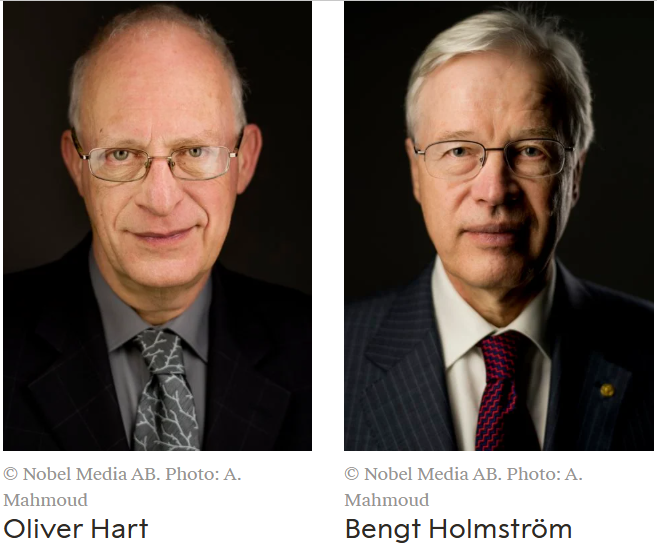
\includegraphics[]{Figure/Hard&Holmstrom_2016NobelPrize.png}
    } %end of resizebox
%-----------------------------------------------
% Figure setting: caption and label
%-----------------------------------------------
%\caption{}
%\label{fig:ModelIntuition_Graphs}
\end{figure}
%-----------------------------------------------

\textbf{2016 Nobel Prize in Economic Science: Award for Hart and Holmstrom}

\vspace{-5mm}
%-----------------------------------------------
\begin{figure}[H]
    \resizebox{5.6in}{0.8in}{%
    %\resizebox{\textwidth}{!}{%
    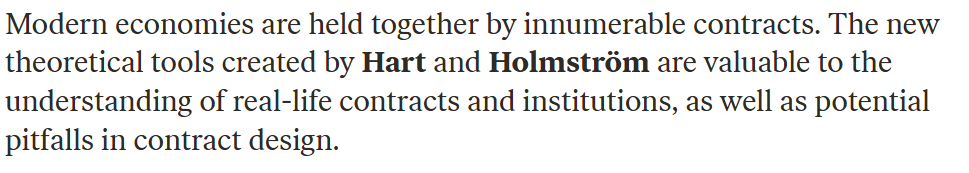
\includegraphics[]{Figure/Hard&Holmstrom_2016NobelPrize_AwardSpeech.png}
    } %end of resizebox
%-----------------------------------------------
% Figure setting: caption and label
%-----------------------------------------------
%\caption{}
%\label{fig:ModelIntuition_Graphs}
\end{figure}
%-----------------------------------------------



\end{frame}

%------------------------------------------------



%------------------------------------------------

\begin{frame}
\frametitle{Moral Hazard}

\textbf{Nobel Prize 2016 (Oliver Hart and Bengt Holmstr\"om)} 
\begin{itemize}
    \item \textbf{Definition}: information or agency problems occurring \textbf{after} a financial transaction
    \item \textbf{Example}: managers take excessive risks or steal outright 
\end{itemize} \pause 

\medskip 

\textbf{Moral Hazard in Equity Contracts: \textcolor{red}{the Principal–Agent Problem}}
\begin{itemize}
    \item \textbf{Equity contracts are subject to the principal–agent problem.}
    \begin{itemize}
        \item The \textbf{principal} is the one whose money is on the line. The \textbf{agent} is the one making the decision. 
        \item In the stock market: when the stockholders (the principals) are not the managers (agent), managers may act in their own interest. \pause 
        \item Example: managers may engage in \textbf{empire-building}, expanding the company beyond its optimal size in order to gain prestige, fame, and private benefits (like a jet plane) 
    \end{itemize}
\end{itemize}




\end{frame}

%------------------------------------------------




%------------------------------------------------

\begin{frame}
\frametitle{Moral Hazard}

\textbf{The Principal–Agent Problem} 
\begin{itemize}
    \medskip 
    \item \textbf{Example 1. Shirking} \pause 
    \begin{itemize}
        \item An ice-cream store has two owners: you invest \$9000 while Steve invests \$1000.
        \item If Steve works hard enough, the profit will be \$50,000 per year. Steve will receive 10\% (\$5,000) and you will receive 90\% (\$45,000).
        \item \$5,000 may not be enough to motivate Steven to work hard enough (shirk).
    \end{itemize}
    \medskip 
    \item \textbf{Example 2. Empire building} \pause 
    \begin{itemize}
        \item managers might also acquire other firms to enhance their personal power but do not increase profitability.
    \end{itemize}
    \medskip 
    \item \textbf{Example 3. Personal use} \pause 
    \begin{itemize}
        \item managers might buy a private jet with company's fund.
    \end{itemize}
\end{itemize}



\end{frame}

%------------------------------------------------



%------------------------------------------------

\begin{frame}
\frametitle{Tools to Help Solve the Principal–Agent Problem}

\textbf{Tool 1. Production of Information: Monitoring} 
\begin{itemize}
    \item \textbf{Monitoring}: auditing the firm and checking on frequently
    \medskip
    \item \textbf{Why monitoring by owners is less efficient}
    \begin{itemize}
        \item \testbf{\textcolor{red}{Costly state-verification}}: the cost of monitoring makes it less frequent and less efficient
        \smallskip 
        \item \textcolor{red}{Free-rider problem}: most owners are less likely to monitor actively 
    \end{itemize}
\end{itemize} \pause 

\medskip 

\textbf{Tool 2. Government Regulation to Increase Information } 
\begin{itemize} 
    \item (1) force \textbf{Generally-Accepted Accounting Principles (``GAAP'')} that make profit verification easier
    \item (2) impose stiff criminal penalties on people who commit fraud.
    \medskip
    \item \textbf{Why Government Regulation cannot eliminate Principal–Agent Problem}
    \begin{itemize}
        \item \testbf{\textcolor{red}{catching fraud is not easy and very costly}}.
    \end{itemize}
\end{itemize}


\end{frame}

%------------------------------------------------






%------------------------------------------------

\begin{frame}
\frametitle{Tools to Help Solve the Principal–Agent Problem}


\textbf{Tool 3. Financial Intermediation} 
    \medskip
\begin{itemize}
    \item \textbf{Private equity} funds are financial intermediaries designed to solve the \textcolor{red}{free-rider problem} 
    \medskip
    \item \textbf{Financial intermediaries' advantages}: \pause 
    \begin{itemize}
        \item privacy: buy whole companies, don't need to disclose trades
        \item economics of scale: reduces costs of monitoring per dollar
        \item expertise: focus on a few sectors such as high-tech
        \item long-term investment horizon: align incentives of entrepreneur and investor  
    \end{itemize} \pause 
    \medskip
    \item \textbf{Example: venture capital firm} \pause 
    \begin{itemize}
        \item pool the resources of their partners and use the funds (as equity) to help budding entrepreneurs start new businesses
        \item monitoring: demand representation in the board of directors
        \item long horizon: wait until IPO or exit by selling to another VC (Uber and Amazon had many years of negative profits)
    \end{itemize}
\end{itemize}


\end{frame}

%------------------------------------------------



%------------------------------------------------

\begin{frame}
\frametitle{Tools to Help Solve the Principal–Agent Problem}


\textbf{Tool 4. Debt Contracts} 
\begin{itemize} 
    \item Suppose that it is \textbf{costly} for the principal to monitor the agent. 
    \item Can we structure a contract so that the principal \textbf{rarely} needs to verify the reports from the agent (this is the theory of Townsend I mentioned)? 
\end{itemize}
\vspace{-2mm}
%-----------------------------------------------
\begin{figure}[H]
    \resizebox{4in}{1in}{%
    %\resizebox{\textwidth}{!}{%
    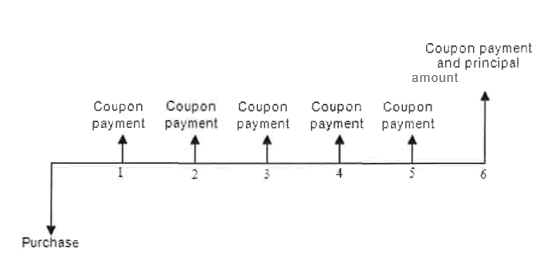
\includegraphics[]{Figure/LongTermDebt_Cashflow.png}
    } %end of resizebox
%-----------------------------------------------
% Figure setting: caption and label
%-----------------------------------------------
%\caption{\scriptsize{Source: Andreas Hackethal and Reinhard H. Schmidt, “Financing Patterns: Measurement Concepts and Empirical Results,” Johann Wolfgang Goethe-Universitat Working Paper No. 125, January 2004. The data are from 1970–2000 and are gross flows as percentage of the total, not including trade and other credit data, which are not available.}}
%\label{fig:ModelIntuition_Graphs}
\end{figure}
%-----------------------------------------------
\begin{itemize}
    \item \textbf{Fixed dollar amounts at periodic intervals}: does not need to monitor as long as periodic payment is satisfied. $\rightarrow$ \textbf{reduces \textcolor{red}{costly state verification}}.
    \begin{itemize}
        \item Only when default occurs, debt holders need \textcolor{red}{costly state verification} and liquidation.
    \end{itemize}
\end{itemize}


\end{frame}

%------------------------------------------------





%------------------------------------------------

\begin{frame}
\frametitle{Moral Hazard Influences Financial Structure in Debt Markets}


Example: Steve’s ice-cream store
\begin{itemize} 
    \medskip 
    \item Steves starts with \$1000 equity, and you lend Steve the \$9,000 as debt. 
    \begin{itemize}
        \item If Steve works hard enough, the profit will be \$50,000   per year. Steve will receive \$40,000, and you will receive \$10,000.
    \end{itemize}
    \medskip 
    \item \textbf{Steve's moral hazard}: might want to invest \$10,000 in highly risky project: chemical research project
    \begin{itemize}
        \item 1-in-10 chance of inventing a diet ice cream and becoming a multimillionaire. You only get \$10,000 %(\textbf{\textcolor{red}{not sharing with success}}).
        \item When failure occurs, both Steve and you get \$0 %(\textbf{\textcolor{red}{undertaking failure}}).
    \end{itemize}
\end{itemize}


\end{frame}

%------------------------------------------------




%------------------------------------------------

\begin{frame}
\frametitle{Tools to Help Solve Moral Hazard Problem in Debt Contracts}


\begin{itemize}
    \item \textbf{Tool 1. Net Worth and Collateral}
    \begin{itemize}
        \item \textbf{Make the debt contract incentive-compatible}: When borrowers have more at stake, moral hazard is greatly reduced. 
        \item Example Steve's ice-cream store: increase Steve's equity
        \begin{itemize}
            \item Now steve's equity is \$910,000 instead of \$10,000. 
            \item If Steve is unsuccessful in chemical machines (prob is 90\%), he will lose \$910,000  instead of \$10,000. $\rightarrow$ He is much less likely to take high risk. 
        \end{itemize}      
    \end{itemize}
    \item \textbf{Tool 2. Monitoring and Enforcement of Restrictive Covenants} 
    \begin{itemize}
        \item \textbf{Discourage undesirable behavior}: (1) debt only finances finance specific activities; (2) restrict from risky business activities, such as purchasing other businesses.
        \item \textbf{Encourage desirable behavior}: maintain minimum holdings of certain assets relative to the firm’s size
        \item \textbf{Keep collateral valuable}: Automobile loan contracts require a minimum amount of collision and theft insurance and prevent the sale of the car
        \item \textbf{Provide information}
        \item \textbf{Drawback}: (1) impossible to restrict all undesirable activities; (2) \textcolor{red}{free-rider problem}
    \end{itemize}
\end{itemize}



\end{frame}

%------------------------------------------------





%------------------------------------------------

\begin{frame}
\frametitle{Tools to Help Solve Moral Hazard Problem in Debt Contracts}

\vspace{-2mm}
\textbf{Tool 3. Financial Intermediation} 
\begin{itemize} 
    \item \textbf{Financial intermediaries avoid \textcolor{red}{free-rider problem} by private Debt}
    \item \textbf{Financial intermediaries' advantages}:
    \begin{itemize}
        \item (1) economics of scale (2) expertise: focus on a few sectors
    \end{itemize}
    \smakllskip
    \item New tech reduces monitoring cost $\rightarrow$  nonbank lenders' market share increases. 
    \begin{itemize}
        \item Rise of FinTech Nonbank Lenders in Paycheck Protection Program (COVID-19): 
    \end{itemize}
\end{itemize}

\vspace{-1mm}
%-----------------------------------------------
\begin{figure}[H]
    \resizebox{4in}{1.8in}{%
    %\resizebox{\textwidth}{!}{%
    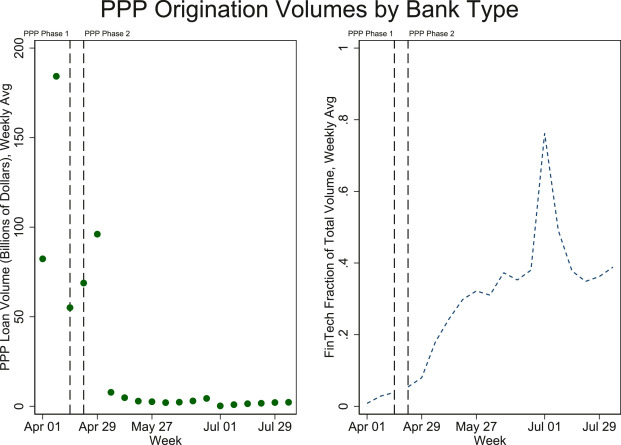
\includegraphics[]{Figure/FinTechNonbankLenders_PPP.jpg}
    } %end of resizebox
%-----------------------------------------------
% Figure setting: caption and label
%-----------------------------------------------
%\caption{\scriptsize{Source: Andreas Hackethal and Reinhard H. Schmidt, “Financing Patterns: Measurement Concepts and Empirical Results,” Johann Wolfgang Goethe-Universitat Working Paper No. 125, January 2004. The data are from 1970–2000 and are gross flows as percentage of the total, not including trade and other credit data, which are not available.}}
%\label{fig:ModelIntuition_Graphs}
\end{figure}
%-----------------------------------------------

\end{frame}

%------------------------------------------------


%----------------------------------------------------------------
%----------------------------------------------------------------
\section{Regulation of the Financial System}
%----------------------------------------------------------------
%----------------------------------------------------------------



%----------------------------------------------------------------
\subsection{Deposit Insurance}
%----------------------------------------------------------------



%------------------------------------------------
\begin{frame}
\frametitle{Regulation of the Financial System}

\textbf{Why Regulation?}
\medskip 
\begin{itemize}
    \item \textbf{To increase the information available to investors}
    \begin{itemize}
        \item Reduce adverse selection and moral hazard problems
    \end{itemize}
    \medskip 
    \item \textbf{To ensure the soundness of financial intermediaries: avoid financial crisis} 
    \begin{itemize}
        \item Restrictions on entry (chartering process)
        \item Disclosure of information (especially risks)
        \item Restrictions on Assets and Activities (control holding of risky assets)
        \item Deposit Insurance (avoid bank runs)
        \item Limits on Competition (mostly in the past): (1) branching; (2) Restrictions on Interest Rates
    \end{itemize}
\end{itemize}
\end{frame}
%------------------------------------------------




%------------------------------------------------
\begin{frame}
\frametitle{Regulation of the Financial System}

\vspace{-6mm}
%-----------------------------------------------
\begin{figure}[H]
    \resizebox{5.6in}{2.9in}{%
    %\resizebox{\textwidth}{!}{%
    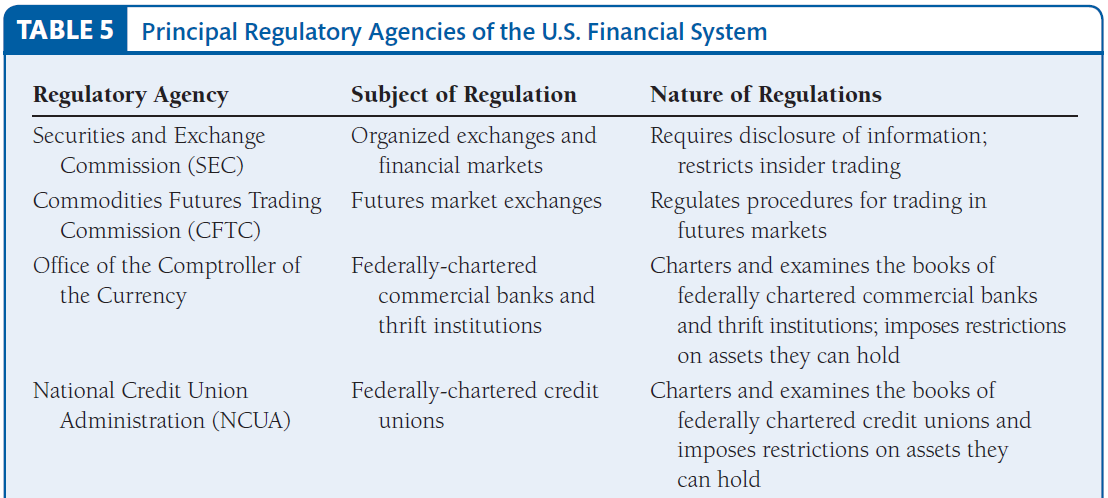
\includegraphics[]{Figure/RegulatoryBodies_PartA.png}
    } %end of resizebox
%-----------------------------------------------
% Figure setting: caption and label
%-----------------------------------------------
%\caption{}
%\label{fig:ModelIntuition_Graphs}
\end{figure}
%-----------------------------------------------


\end{frame}
%------------------------------------------------




%------------------------------------------------
\begin{frame}
\frametitle{Regulation of the Financial System}

\vspace{-6mm}
%-----------------------------------------------
\begin{figure}[H]
    \resizebox{5.6in}{2.9in}{%
    %\resizebox{\textwidth}{!}{%
    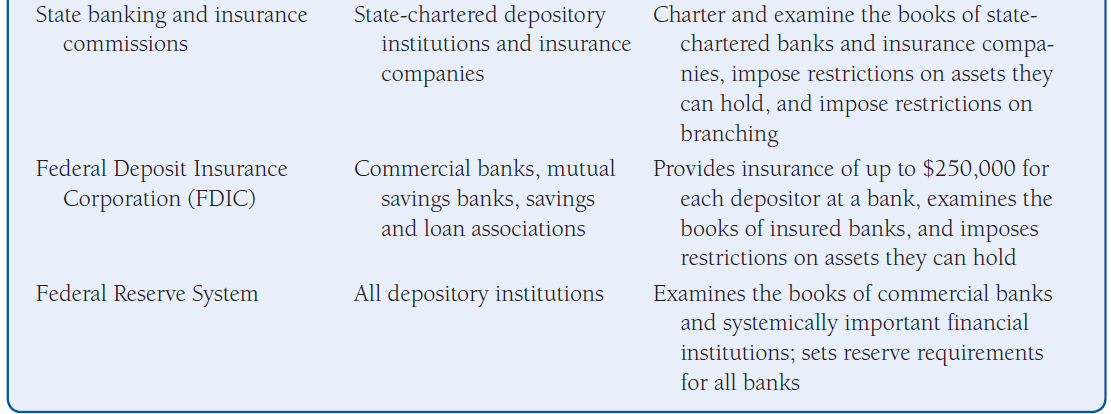
\includegraphics[]{Figure/RegulatoryBodies_PartB.png}
    } %end of resizebox
%-----------------------------------------------
% Figure setting: caption and label
%-----------------------------------------------
%\caption{}
%\label{fig:ModelIntuition_Graphs}
\end{figure}
%-----------------------------------------------


\end{frame}
%------------------------------------------------





%------------------------------------------------

\begin{frame}
\frametitle{\large{Bank and Financial Crisis: Bernanke, Diamond, and Dybvig won 2022 Nobel Prize}}



\vspace{-2mm}
%-----------------------------------------------
\begin{figure}[H]
    \resizebox{3.6in}{1.6in}{%
    %\resizebox{\textwidth}{!}{%
    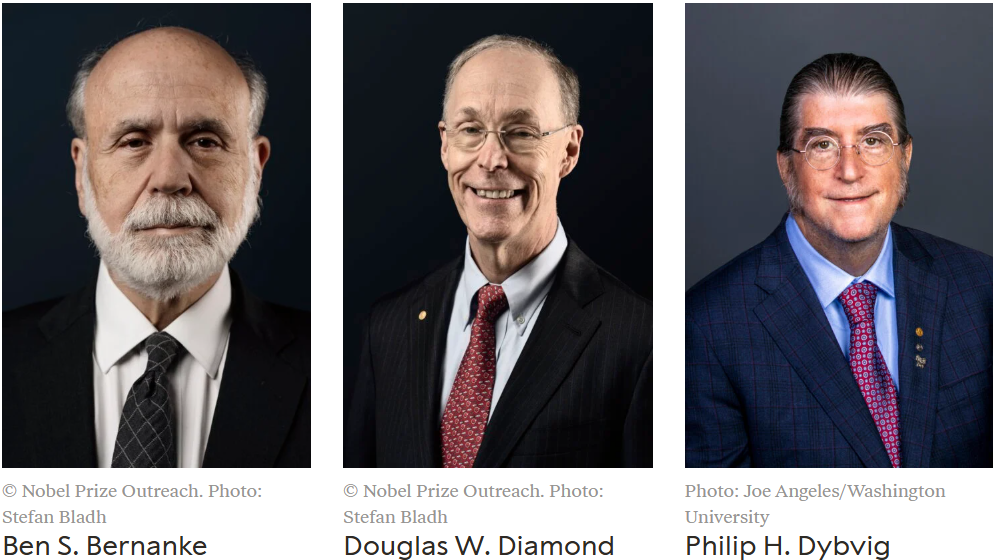
\includegraphics[]{Figure/BernankeDiamond&Dybvig_2022NobelPrize.png}
    } %end of resizebox
%-----------------------------------------------
% Figure setting: caption and label
%-----------------------------------------------
%\caption{}
%\label{fig:ModelIntuition_Graphs}
\end{figure}
%-----------------------------------------------


\vspace{-5mm}
%-----------------------------------------------
\begin{figure}[H]
    \resizebox{4.6in}{1.2in}{%
    %\resizebox{\textwidth}{!}{%
    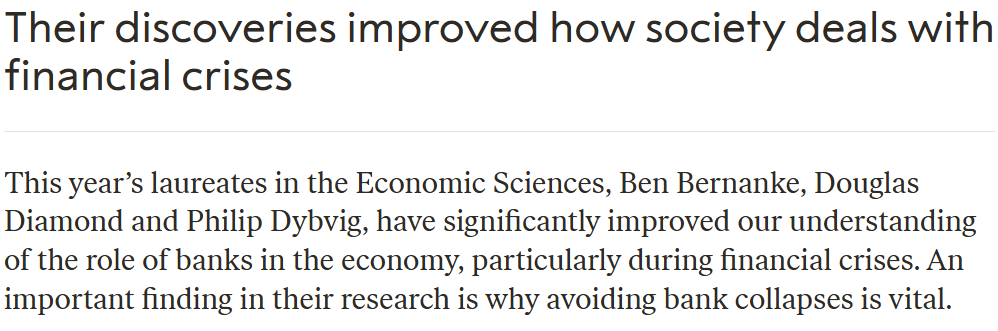
\includegraphics[]{Figure/BernankeDiamond&Dybvig_2022NobelPrize_AwardSpeech.png}
    } %end of resizebox
%-----------------------------------------------
% Figure setting: caption and label
%-----------------------------------------------
%\caption{}
%\label{fig:ModelIntuition_Graphs}
\end{figure}
%-----------------------------------------------



\end{frame}

%------------------------------------------------






%------------------------------------------------
\begin{frame}
\frametitle{Deposit Insurance}

\textbf{Rational of Deposit Insurance for Banks}: Diamond and Dybvig (1983) won Economic Nobel Prize in 2022
\medskip 
\begin{itemize}
    \item \textbf{Banks: channel money from savers to borrowers}
    \begin{itemize}
        \item savers (both households and firms): have idle money but may need money at any time due to unforeseen expenditures. Savers prefer a liquid account that allows for withdraw at any time. 
        \item borrowers (firms): need loans for long-term investment.
    \end{itemize}
    \medskip 
    \item \textbf{Under ordinary circumstances, banks can run businesses and earn profits safely} 
    \begin{itemize}
        \item Savers' unpredictable needs for cash are likely to be random and unlikely happen at the same time. 
        \item Banks need some reserve to cover random and small-size withdraw. 
    \end{itemize}
\end{itemize}
\end{frame}
%------------------------------------------------





%------------------------------------------------
\begin{frame}
\frametitle{Deposit Insurance}

\textbf{Rational of Deposit Insurance for Banks}: Diamond and Dybvig (1983) won Economic Nobel Prize in 2022
\medskip 
\begin{itemize}
    \item \textbf{Banks' key constraint: cannot hold all money as reserve}
    \begin{itemize}
        \item When many savers withdraw, banks are sure to fail since long-term loans cannot be returned immediately. Banks can only afford withdraw of first-come savers. 
    \end{itemize}
    \medskip 
    \item Situations when many savers withdraw
    \begin{itemize}
        \item Big aggregate shocks: natural disasters, wars, economic recessions
        \item \textbf{\textcolor{red}{``bank run" as Self-fulfilling prophecy}: When many savers believe other savers will withdraw (say a rumor), savers all have an incentive to rush to be the first in line to withdraw their funds.}
    \end{itemize}
    \medskip 
    \item Given extremely bad recessions caused by bank failure, the most efficient method to avoid ``bank run" is to provide \textbf{\textcolor{red}{deposit insurance}} by the Federal Reserve. 
\end{itemize}
\end{frame}
%------------------------------------------------

%--------------------------------------------------------------------
\subsection{Why do banking crises (on paper) create (real) economic recessions?}
%--------------------------------------------------------------------


%------------------------------------------------
\begin{frame}
\frametitle{Why do banking crises (on paper) create (real) economic recessions?}

\textbf{Bernanke (1983): \textcolor{red}{Some Banks' valuable knowledge is lost in a crisis.}}
\medskip 
\begin{itemize}
    \item \textbf{Banks take time to build knowledge capital about their customers}
    \begin{itemize}
        \item Are the borrowers good at business? Are borrowers working hard and being honest? 
    \end{itemize}
    \medskip 
    \item \textbf{In normal economic conditions}: 
    \begin{itemize}
        \item Bank A has built knowledge capital about corporate X1, X2, and X3. 
        \item Bank B has built knowledge capital about corporate Y1, Y2, and Y3.
    \end{itemize}
    \medskip 
    \item \textbf{In a banking crisis (even no economic crisis), Bank A fails.} $\rightarrow$ Corporate X1, X2, and X3 cannot get enough funds as Bank B has no knowledge of them even if
    \begin{itemize}
        \item Corporate X1, X2, and X3 have good projects, working hard, and being honest. 
        \item Bank B has enough money. 
    \end{itemize}
\end{itemize}

\medskip 

Summary: \textbf{\textcolor{red}{In this banking crisis, Bank A's lost knowledge as a financial friction that prevents economic runs (produces) at its full capacity}}
\end{frame}
%------------------------------------------------




%------------------------------------------------
\begin{frame}
\frametitle{Why do Financial Frictions Create Economic Recession?}
\vspace{-2mm}
\textbf{Bernanke, Getler, and Gilchrist (1999): \textcolor{red}{Financial Accelerator: Collateral-based borrowing constraint tightens in a crisis + positive feedback loop}}


\begin{itemize}
    \item The corporate borrowing constraint is often tightened by collateral value to reduce bad results due to asymmetric information. 
\end{itemize}


\vspace{-2mm}
%-----------------------------------------------
\begin{figure}[H]
    \resizebox{5in}{1.8in}{%
    %\resizebox{\textwidth}{!}{%
    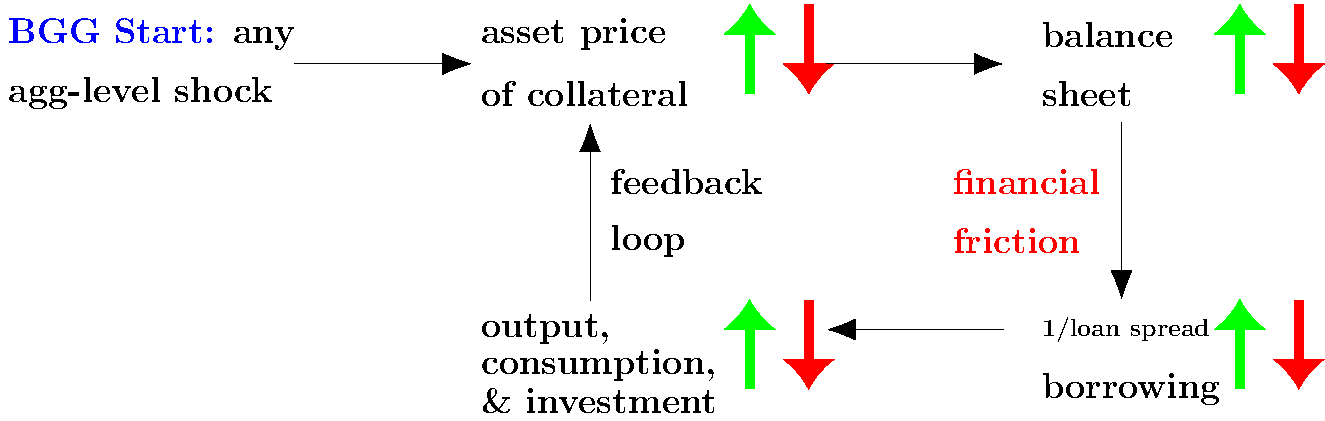
\includegraphics[width=0.9\textwidth]{Figure/BGG1999_Intuition.pdf}
    } %end of resizebox
%-----------------------------------------------
% Figure setting: caption and label
%-----------------------------------------------
%\caption{Source: Xiangyang Li's lecture notes P11}
%\label{fig:ModelIntuition_Graphs}
\end{figure}
%-----------------------------------------------


\end{frame}
%------------------------------------------------





%------------------------------------------------
\begin{frame}
\frametitle{Why do Banking Crises Create Economic Recessions?}
\vspace{-2mm}


\textbf{BGG (1999) also explains another mechanism: \textcolor{red}{banking crisis alone can cause economic recession}}



\vspace{-2mm}
%-----------------------------------------------
\begin{figure}[H]
    \resizebox{5in}{1.8in}{%
    %\resizebox{\textwidth}{!}{%
    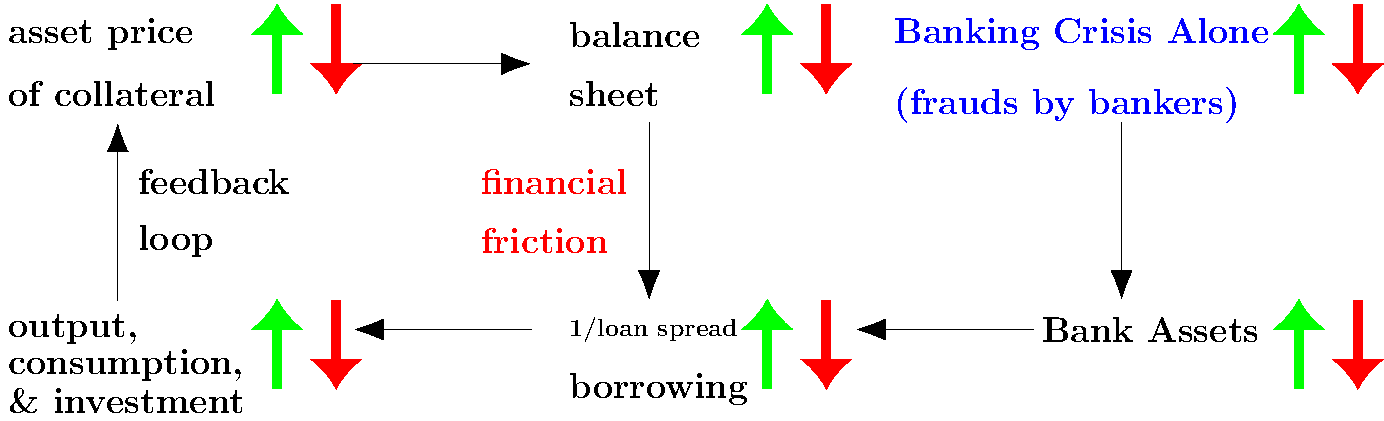
\includegraphics[width=0.9\textwidth]{Figure/WhyBankCrisisAlongCanCauseEconomicRecession.pdf}
    } %end of resizebox
%-----------------------------------------------
% Figure setting: caption and label
%-----------------------------------------------
%\caption{Source: Xiangyang Li's lecture notes P11}
%\label{fig:ModelIntuition_Graphs}
\end{figure}
%-----------------------------------------------


Based on this research, Bernanke, as the chairman of the Federal Reserve, insisted that the U.S. government needed to bail out banks in the 2008 Financial Crisis.

\end{frame}
%------------------------------------------------



%---------------------------------------------------------------------
%---------------------------------------------------------------------

\appendix
% (1)	The slides in the appendix will not count towards the total slide number that is displayed for the normal slides. Backup slides will have their own slide numbers and total slide numbers counted anew from the start of the appendix. Very handy! 
%(2)	You can organize your backup slides in sections, these section will not appear in the table of content. 
%------------------------------------------------




\end{document}